% Created 2018-01-18 Thu 22:19
% \documentclass[aspectratio=169,10pt,trans]{beamer}
% \documentclass[aspectratio=169,10pt,trans]{beamer}
\documentclass[aspectratio=169,10pt]{beamer}

%% for handouts mode
%\documentclass[aspectra§tio=169,10pt,handout]{beamer}
%%%% Definitions
\def\ppttitle{The Pendulum Turn: Are Rally Drivers Wrong?}
\def\pptshorttitle{PEP}
\def\authfull{Arvind Balachandran}
\def\authshort{Arvind}
\def\unversityname{Linköping University}
\def\affiliationtitle{Devision of Vehicular Systems\\
Department of Electrical Engineering}

% LiU theme packages
\usepackage{myLiU}%\usetheme{Madrid}
\usepackage[utf8]{inputenc}
\usepackage[T1]{fontenc}
%\usepackage{fixltx2e}
\usepackage{graphicx}
\usepackage{xcolor}
%\usepackage{longtable}
\usepackage{float}
%\usepackage{wrapfig}
%\usepackage{rotating}
\usepackage{fontawesome5}
% \usepackage[normalem]{ulem}
\usepackage{amsmath}
%\usepackage{textcomp}
% \usepackage{marvosym}
% \usepackage{wasysym}
\usepackage{amssymb}
\usepackage{hyperref}
\usepackage[round]{natbib}
\usepackage{color}
\usepackage{listings}
\lstset{language=Matlab,%
  % basicstyle=\color{red},
  breaklines=true,%
  morekeywords={matlab2tikz},
  keywordstyle=\color{blue},%
  morekeywords=[2]{1}, keywordstyle=[2]{\color{black}},
  identifierstyle=\color{black},%
  stringstyle=\color{mylilas},
  commentstyle=\color{mygreen},%
  showstringspaces=false,%without this there will be a symbol in the places where there is a space
  numbers=left,%
  numberstyle={\tiny \color{black}},% size of the numbers
  numbersep=5pt, % this defines how far the numbers are from the text
  emph=[1]{for,end,break},emphstyle=[1]\color{red}, %some words to emphasise
  % emph=[2]{word1,word2}, emphstyle=[2]{style},    
}

% \usepackage{array} % package for tables

\tolerance=1000
% \usetheme{default}
\author[\authshort]{\authfull}
\date{\today}
\title[\pptshorttitle]{\ppttitle}
\titlegraphic{\pgfuseimage{titlegraphic}}
\institute[\unversityname]{\affiliationtitle}
%\hypersetup{
%  pdfkeywords={},
%  pdfsubject={}}

% \usepackage{siunitx}

%-------------------------------------------
% Handouts 
%\usepackage{handoutWithNotes}
%\pgfpagesuselayout{4 on 1 with notes}[a4paper,border shrink=5mm]
% \AtBeginSection[\star] % Do nothing for \section*
% {
% \begin{frame}<beamer>
% \frametitle{Outline}
% \tableofcontents[currentsection]
% \end{frame}
% }
% temperorily disable overlays
%\newcommand*{\disableanim}[1]{{%
%		\RenewDocumentCommand{\onslide}{ R<>{} }{}%
%		#1%
%}}
% \setbeamercolor{section in toc}{fg=black}
% \setbeamercolor{subsection in toc}{fg=black}
% \setbeamercolor{part in toc}{fg=black}

% \usepackage{tikz}
% \usepackage{pgf-pie}  
\AtBeginPart{\frame{\partpage}}

\setbeamertemplate{section page}{  
  \begingroup    
  \centering
  \begin{beamercolorbox}[sep=12pt,center,colsep=-4bp,rounded=true,shadow=flase]{section title}       
    \usebeamerfont{section title}\insertsection\par     
  \end{beamercolorbox}   
  \endgroup 
}
\AtBeginSection{\frame{\sectionpage}}

%% notes package
% \usepackage{pgfpages}
% \setbeameroption{show notes}
% \setbeameroption{show notes on second screen=right}

%% Animation package 
\usepackage{animate}

\usepackage{layouts}

\begin{document}

\maketitle

% \part[PEP-1]{PEP:Part 1}

% \section{Problem Formulation}
\begin{frame}{Problem Statement}
    \begin{alertblock}{PEP: Pendulum Turn}
        Experiment with vehicle parameters (especially inertia) to see if it occurs. (Are many rally drivers wrong?)
    \end{alertblock}
    \pause
    \begin{exampleblock}{}
        Cost functions:
        \begin{align*}
            J &= \begin{cases} 
                    \text{Min }\quad t + 0.1\left(\beta_x + \beta_y\right) & \text{min } t \\
                    \text{Max }\quad v_x(t_f) + 0.1\left(\beta_x + \beta_y\right) & \text{max } v_f 
                 \end{cases}.
        \end{align*}
    \end{exampleblock}
    \begin{align*}
        & \text{subject to} 
        & & \dot x = f(x,u), && \text{ODE}\\
        &&& f_u(u) \leq 0 && \text{Constraints}\\
    %
        &&& f_o(x,u) \leq 0 && \text{Path} \\
    %
        &&& x_0,\ x_f, && \text{Initial values}
    \end{align*}
\end{frame}
% \begin{frame}
    \frametitle{ST-model with Pacejka friction ellipses}
    \begin{block}{}
        \begin{description}
            \item[States:] 9, $X_p,\ Y_p,\ \psi,\ v_x,\ v_y,\ r,\ \delta,\ F_{x(f)},\ F_{x(r)}$
            \item[Inputs:] 3, $\dot \delta,\ F_{x(f)}^*,\ F_{x(r)}^*$
        \end{description}
    \end{block}
    \vspace{10pt}
    \pause
    \begin{columns}
        \begin{column}{0.45\textwidth}
            Also the friction ellipses 
            \begin{align*}
                F_{y(i)} &= F_{y0(i)}\left(\alpha_i\right)\sqrt{1 - \left(\frac{F_{x(i)}}{F_{x0(i)}^{\text   {max}}}\right)}
            \end{align*}
        \end{column}\pause
        \begin{column}{0.45\textwidth}
            Note that $F_{x(f)}^*,\ F_{x(r)}^*$ are used to generate $F_{x(f)},\ F_{x(r)}$ using
            \begin{align*}
                \dot F_{x(i)} = \frac{1}{\tau_f}\left(F_{x(i)} - F_{x(i)}^*\right)
            \end{align*}
        \end{column}
    \end{columns}
    \vspace{10pt}
    \begin{alertblock}{}
        The dangerous \textbf{sqaure root} causes a lot of trouble in optimization.
    \end{alertblock}
\end{frame}
% \begin{frame}{Constraints and more}
    \begin{columns}
        % \begin{column}{0.4\textwidth}
        %     \textbf{Constraints}
        %     \begin{align*}
        %         -\delta_{\text{max}} &\leq \delta \leq \delta_{\text{max}},\\
        %         -\dot\delta_{\text{max}} &\leq \dot\delta \leq \dot\delta_{\text{max}},\\
        %         -F_{x(f),\text{max}} &\leq F_{x(f)} \leq F_{x(f),\text{max}},\\
        %         -F_{x(r),\text{max}} &\leq F_{x(r)} \leq 0,\\
        %         -F_{x(f),\text{max}} &\leq F_{x(f)}^* \leq F_{x(f),\text{max}},\\
        %         -F_{x(r),\text{max}} &\leq F_{x(r)}^* \leq 0,\\
        %         v_x &> 0\\
        %         0 &\leq \beta_x \leq 1\\
        %         0 &\leq \beta_y \leq 1,
        %     \end{align*}
        % \end{column}
        \begin{column}{0.3\textwidth}
            \textbf{Hairpin}
            \begin{align*}
                \left(\frac{x-X_\text{a}}{R_1^i}\right)^n + \left(\frac{y}{R_2^i}\right)^n & \geq 1, \\
                \left(\frac{x-X_a}{R_1^o}\right)^n + \left(\frac{y}{R_2^o}\right)^n & \leq 1.
            \end{align*}
            
            \vspace{10pt}
            \textbf{Slack Variables}
            \begin{align*}
                0 \leq \beta_x &\leq 1,\\
                0 \leq \beta_y &\leq 1,\\
                x_f - \beta_y, \leq X_p(t_f) &\leq x_f + \beta_x,\\
                y_f - \beta_y, \leq Y_p(t_f) &\leq y_f + \beta_y,
            \end{align*}
        \end{column}
        \begin{column}{0.2\textwidth}
            \begin{tabular}{c|c}
                Parameter & Value \\
                \hline
                $\delta_{\text{max}}$ & 30$^\circ$ \\
                $\dot \delta_{\text{max}}$ & 45$^\circ$/s\\
                $\tau_f$ & 0.1\,s\\
                $X_a$ & 10\,m\\
                $R_1^i$ & 2\,m\\
                $R_2^i$ & 50\,m\\
                $R_1^o$ & 7\,m\\
                $R_2^o$ & 55\,m\\
                $n$ & 4\\
                \hline
                $m$ & 2100\,kg\\
                $l_f$ & 1.3\,m\\
                $l_r$ & 1.5\,m\\
                $g$ & 9.82\,m/s\textsuperscript{2}\\
                $I_{zz}$ & 3900\,Kgm\textsuperscript{2}\\
            \end{tabular}
        \end{column}
    \end{columns}
\end{frame}
% \begin{frame}{Optimization procedure}
    \begin{columns}
        \begin{column}{0.5\textwidth}
            \begin{block}{The Älgorithm}
                \begin{enumerate}
                    \item Begin with simple problem, $R_{2} = 1$\,m.
                    \item Store the optimized results and use them as initial guesses in the next iteration.
                    \item Increase the length of the hairpin and optimize.
                \end{enumerate} 
            \end{block}    
            \begin{alertblock}{Risk}
                The risk of converging into local minima is quite high.
            \end{alertblock}    
        \end{column}
        \begin{column}{0.3\textwidth}
            \includegraphics{figures/inc_opti_alg.pdf}
        \end{column}
    \end{columns}
\end{frame}
\begin{frame}{Some Results}
    \begin{columns}
        \begin{column}{0.3\textwidth}
            \centering
            \includegraphics[width=0.9\textwidth]{figures/pep1_part1.pdf}
        \end{column}
        \begin{column}{0.55\textwidth}
            Always interesting to see Arvind diagrams.
            \includegraphics[width=\textwidth]{figures/pep1_part1_arp.pdf}        
            \begin{alertblock}{}
                Seems like the pendulum turn is the optimal solution when the goal is to maximize exit velocity.
            \end{alertblock}
        \end{column}
    \end{columns}
\end{frame}
\begin{frame}{Let's talk numbers}
    \begin{table}
        \centering
        \begin{tabular}{c|c|c}
            & $t_f$ & $v_f$\\
            \hline
            (topt) Min $t_f$ & 7.83\,s & 25.11 m/s (90.4\,km/h)\\
            (vopt) Max $v_f$ & 8.84\,s & 26.68 m/s (96\,km/h)\\
        \end{tabular}
    \end{table}
    \pause
    Relative velocities of the two scenarios, vopt is 1.57 m/s faster at $Y_p = 0$\,m.
    \pause

    Assuming equal acceleration for both cases, will the vopt vehicle catch up to topt? \pause
    \vfill
    \begin{columns}
        \begin{column}{0.7\textwidth}
            \begin{figure}
                \centering
                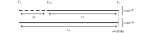
\includegraphics[width=\textwidth]{figures/pep1_analys.pdf}
            \end{figure} \pause
        \end{column}
        \begin{column}{0.3\textwidth}
            Assuming a point mass model.
            \begin{alertblock}{}
                Yes! If $V_{T0} < V_{yo(V)}$, i.e., $\mu < 0.158$. \newline
                So icy conditions at the end of the hairpin?
            \end{alertblock}
        \end{column}
    \end{columns}

\begin{exampleblock}{}
    For the pendulum term to be "\textit{viable}", $V_{T0} < V_{yo(V)}$. In other words, the topt solution?
\end{exampleblock}

\end{frame}
% \begin{frame}{PEP 2: Hairpin turn continuation}
    \begin{alertblock}{Comparing different models}
        Can we see the pendulum turn in the PM?
    \end{alertblock}

    \begin{alertblock}{Improved ST model}
        Introducing the wheel dynamics and using weighted functions for the tire model. 

        Include load transfer.
    \end{alertblock}

    \begin{alertblock}{Road Frictions}
        Exploring the pendulum turn and minimum time turn at different road frictions.
    \end{alertblock}

    \begin{alertblock}{Calculating the Racing line and track layout}
        What is the racing line through the hairpin? 

        Is the pendulum turn an optimal solution for a 90$^\circ$ curve?
    \end{alertblock}

\end{frame}
\begin{frame}{Houston, we have a problem}
    \begin{columns}
        \begin{column}{0.5\textwidth}
            The hairpin turn maneuver is difficult to find a solution.

            \begin{alertblock}{400 Bad Request}
                \begin{itemize}
                    \item[\faSkullCrossbones] \texttt{Restoration Failed.}
                    \item[\faSkullCrossbones] \texttt{Solver encountered NaN.}
                    \item[\faSkullCrossbones] \texttt{Problem may be infeasable.}
                \end{itemize}
            \end{alertblock}

            Challenging to re-create the results. \\
            Very sensitive to the initial conditions (initial guesses). 
        \end{column}
        \begin{column}{0.5\textwidth} \pause
            A right-hand turn maneuver easier to find a solution.

            \begin{block}{So what's good}
                \begin{itemize}
                    \item No need for homotopic.
                    \item Fast computation time.
                \end{itemize}
            \end{block}
        \end{column}
    \end{columns}

    \pause
    \begin{exampleblock}{}
        The investigation hereafter considers a right-hand turn maneuver for the ST-model with load transfer.
    \end{exampleblock}

\end{frame}
\begin{frame}{Some results}
    Still talking numbers.
    \begin{table}[h!]
        \centering
        \begin{tabular}{c|c|c|c|c|c|c|c}
            & & \multicolumn{2}{c|}{Dry Asphalt} & \multicolumn{2}{c|}{Wet Asphalt} & \multicolumn{2}{c}{Snow}\\
            & & $t_f$ & $v_f$ & $t_f$ & $v_f$ & $t_f$ & $v_f$\\
            \hline
            \textbf{topt} & Min $t_f$ & 6.64\,s & 29.1 m/s & 6.86\,s & 27.68\,m/s & 10.9\,s & 17.64\,m/s\\
            & & & 104.77\,km/h & & 99.65\,km/h & & 63.49\,km/h\\
            \textbf{vopt} & Max $v_f$ & 8.15\,s & 29.66 m/s & 7.94\,s & 28.23\,m/s & 11.77\,s & 18.18\,m/s\\
            & & & 106.78\,km/h & & 101.69\,km/h & & 65.43\,km/h\\
        \end{tabular}
    \end{table}
    \pause
    \begin{block}{}
        The velocity optimized is still "\textit{slower}" than the time optimized
    \end{block}

    However$\dots$
\end{frame}
\begin{frame}{We Have Hope}
    \subtitle{"Rebellions Are Built On Hope!"}
    Similar time- and velocity-optimized trajectories for snow conditions.

    \begin{figure}
        \centering
        \includegraphics[height=0.7\textheight]{figures/pep2_iceice.pdf}
    \end{figure}

    % \begin{exampleblock}{}
    %     Is this a clue? Maybe!  
    % \end{exampleblock}

\end{frame}

% \begin{frame}{Sizes}
%   The width of a column is:
%   \printinunitsof{mm}\prntlen{\textwidth} (\printinunitsof{in}\prntlen{\textwidth}) \\
%   The height of a column is:
%   \printinunitsof{mm}\prntlen{\textheight} (\printinunitsof{in}\prntlen{\textheight}) \\  
% \end{frame}

% \include{frames/}
\end{document}
%%% Local Variables:
%%% mode: latex
%%% TeX-master: t
%%% End:

